\documentclass{article}[a4paper,12pt]
\usepackage{pst-knot} % For drawing knots
\usepackage{graphicx} % For including images
\usepackage{amsmath} % For math typesetting if needed
\usepackage{amssymb} % For mathfrak if used for H
\usepackage{hyperref} % For clickable URLs and cross-references
\hypersetup{
    colorlinks=true,
    linkcolor=blue,
    filecolor=magenta,
    urlcolor=cyan,
    pdftitle={Knots, Arithmetic Torsion, and Cyclotomic Fields},
    pdfpagemode=FullScreen,
    }
\usepackage{booktabs}   % For professional looking table lines (toprule, midrule, bottomrule)
\usepackage{array}      % For \newcolumntype, enabling custom column definitions
\usepackage[a4paper, margin=1in]{geometry} % Page margin settings, adjust as needed

\title{Knots, Arithmetic Torsion, and Cyclotomic Fields}
\author{Mingli Yuan, Gemini, ChatGPT}
\date{\today}

\begin{document}

\maketitle

\begin{abstract}
This document explores an arithmetic interpretation of knot group theory, focusing on the relationship between knot relators, their corresponding Alexander polynomials, and a newly defined measure termed global arithmetic torsion. By mapping knot group generators to specific arithmetic operations involving a parameter $t$, we demonstrate how the closure condition of a relator path can yield the Alexander polynomial equation $\Delta(t)=0$. Furthermore, the global arithmetic torsion of such paths, $\tau(\gamma_R)(t)$, exhibits a remarkable structure, consistently factoring into the Alexander polynomial $\Delta(t)$ and a cyclotomic component of the form $t^K-1$. This suggests a deep connection between knot topology, the non-commutative nature of arithmetic operation sequences, and algebraic properties related to roots of unity and cyclotomic fields. Examples, including the figure-eight knot ($4_1$) and knots $6_2$ and $6_3$, are used to illustrate these findings.
\end{abstract}

\tableofcontents

\section{Introduction}

Knot theory, a branch of topology, studies mathematical knots, which are embeddings of a circle in 3-dimensional Euclidean space. A fundamental invariant associated with a knot is its Alexander polynomial, $\Delta(t)$, a Laurent polynomial in a variable $t$ with integer coefficients. Knot groups, the fundamental groups of knot complements, provide another powerful algebraic invariant. These groups are often presented in terms of generators and relators.

This work investigates an arithmetic interpretation of knot group operations. By mapping the generators of a knot group to specific arithmetic operations (typically multiplication by a parameter $t$ and addition of unity) acting within an arithmetic expression space, we can translate knot group relators into sequences of arithmetic operations, forming what we call "relator paths." The condition that such a path corresponds to the identity element in the knot group imposes constraints on the parameter $t$.

A key concept explored herein is ``arithmetic torsion.'' Arithmetic operations, such as addition and multiplication, are fundamental. When sequenced, their order of application can significantly alter the outcome; for instance, $(x+c_1) \cdot t \neq (x \cdot t) + c_1$ in general. This failure to commute is a basic form of non-commutativity. For a simple pair of operations, this effect can be quantified locally. When considering an entire path composed of a sequence of arithmetic operations, these non-commutative effects can accumulate.

We introduce \textbf{global arithmetic torsion}, denoted $\tau(\gamma)$, for a given arithmetic path $\gamma$. It is defined as the difference between the standard evaluation of the path, $\nu(\gamma)$, and the evaluation of a "reversed-sequence path," $\nu(\bar{\gamma})$, where the literal operations of $\gamma$ are applied in the exact reverse order:
\[ \tau(\gamma)(t) = \nu(\gamma)(t) - \nu(\bar{\gamma})(t) \]
A vanishing global arithmetic torsion, $\tau(\gamma)(t)=0$, implies that the path $\gamma$ and its reversed-sequence counterpart $\bar{\gamma}$ yield the same result under evaluation with parameter $t$, suggesting an "effective commutativity" for the overall path under these specific conditions.

This document demonstrates through examples that for paths $\gamma_R$ derived from knot relators:
\begin{enumerate}
    \item The condition for the path to effectively act as identity often leads directly to the Alexander polynomial equation $\Delta(t)=0$.
    \item The global arithmetic torsion $\tau(\gamma_R)(t)$ for these paths exhibits a consistent structure, often factoring into $\Delta(t)$ and a term $t^K-1$, where $K$ is an integer. This latter term brings roots of unity and cyclotomic fields into the picture, providing additional conditions under which the torsion vanishes.
\end{enumerate}
These findings suggest a novel link between knot topology, the algebraic structure of arithmetic operations, and number-theoretic concepts.

\section{Arithmetic Interpretation of Knot Relators and the Alexander Polynomial: The $4_1$ Knot Example}

The figure-eight knot, denoted $4_1$, is a fundamental example in knot theory. Its group presentation can be given with:
\begin{itemize}
    \item Generators: $a, b$
    \item Relator: $abbbaBAAB = 1$ (where $A=a^{-1}, B=b^{-1}$)
    \item Alexander polynomial: $\Delta_{4_1}(t) = t^2 - 3t + 1$
\end{itemize}

\begin{figure}[h]
    \centering
    \begin{pspicture}(-2,-2)(2,2)
        \psKnot[linewidth=3pt,linecolor=blue](0,0){4-1} % Draws the 4_1 knot
    \end{pspicture}
    \caption{The Figure-Eight Knot ($4_1$)}
    \label{fig:knot_4_1}
\end{figure}

In the framework of arithmetic expression geometry, we can interpret the generators and their inverses as operators acting within an arithmetic expression space $\mathfrak{H}$. We establish the following mapping, linking the knot group structure to arithmetic operations involving an indeterminate variable $t$ (associated with the Alexander polynomial):
\begin{itemize}
    \item $a \mapsto \otimes_t$ (multiplication by $t$)
    \item $b \mapsto \oplus_1$ (addition of 1)
    \item $A = a^{-1} \mapsto \oslash_t$ (division by $t$, i.e., multiplication by $t^{-1}$)
    \item $B = b^{-1} \mapsto \ominus_1$ (subtraction of 1)
\end{itemize}
Under this interpretation, the relator $abbbaBAAB$ corresponds to a closed loop path (a specific threadlike expression) in the space $\mathfrak{H}$.

\begin{figure}[h]
    \centering
    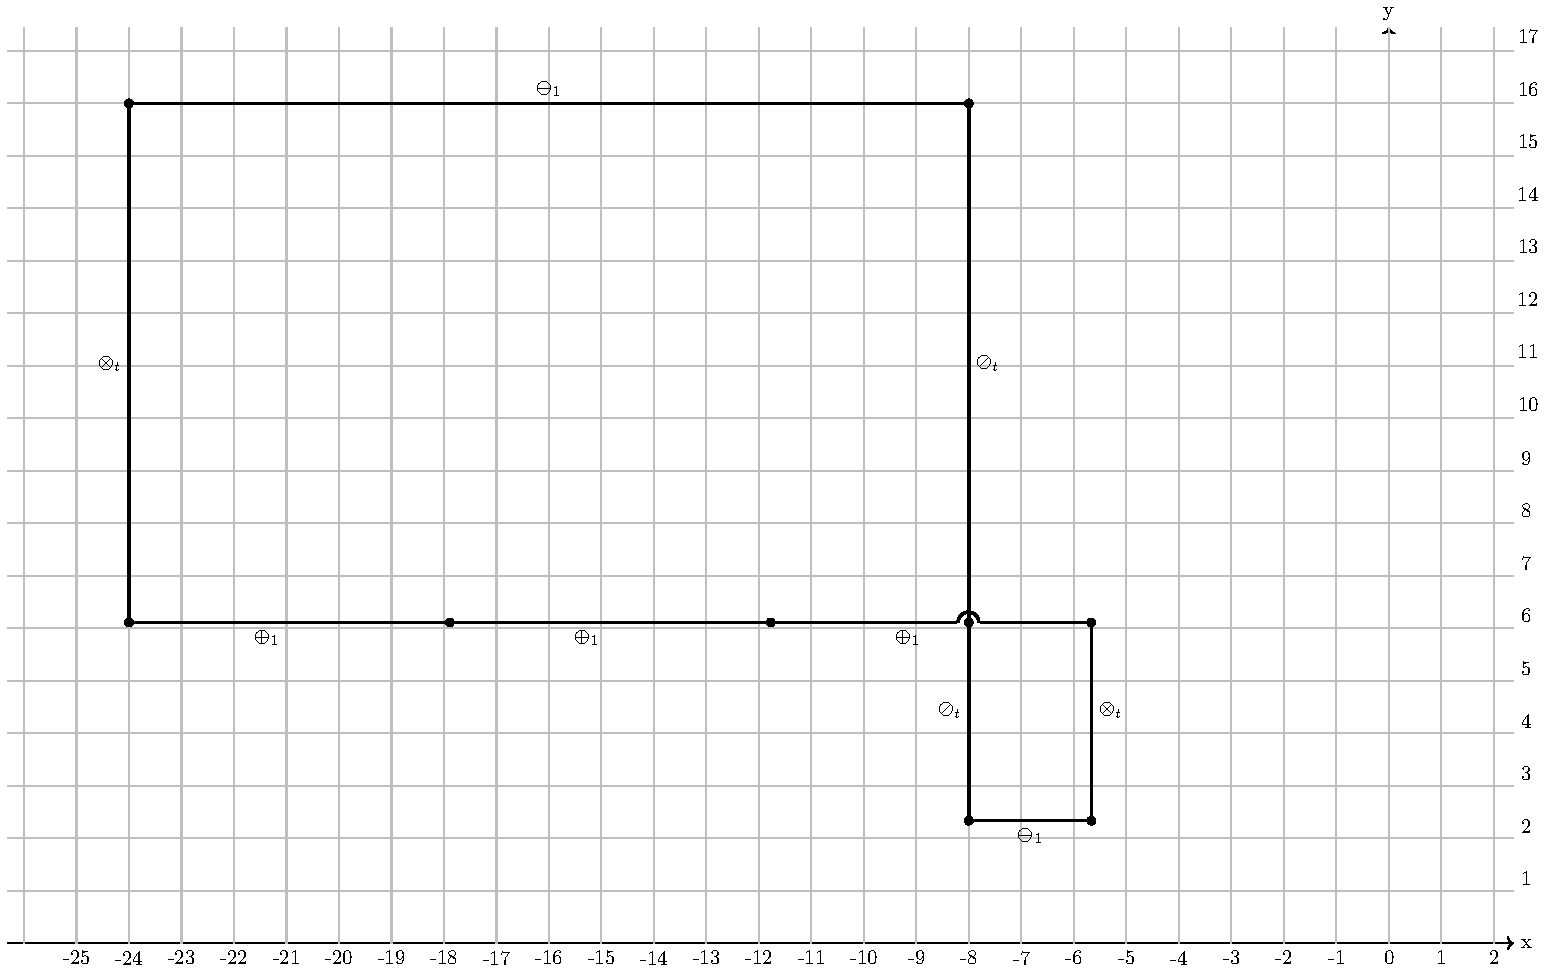
\includegraphics[width=0.8\textwidth]{images/knot_4_1}
    \caption{Schematic representation of the relator path in the arithmetic expression space $\mathfrak{H}$}
    \label{fig:relator}
\end{figure}

Applying the sequence of operators corresponding to the relator $abbbaBAAB$ to a real number $x$ (acting from right to left, consistent with function composition) yields:
\begin{align*}
    \text{Result} &= a(b(b(b(a(B(A(A(B(x))))))))) \\
    &= (x - 1) - t^2 + 3t \\
    &= x - (t^2 - 3t + 1)
\end{align*}
Since the relator $abbbaBAAB$ is equal to the identity element in the knot group, the corresponding path acting on $x$ must return $x$. Therefore, we must have:
\[
x - (t^2 - 3t + 1) = x
\]
This forces the condition $t^2 - 3t + 1 = 0$, which is precisely the Alexander polynomial $\Delta_{4_1}(t)$ of the knot $4_1$ set to zero.

\subsection{Computational Verification for Other Knots}

This observed connection between the knot relator (interpreted arithmetically) and the Alexander polynomial equation $\Delta(t)=0$ is not unique to the knot $4_1$. As previously noted, computational checks for knots up to 11 crossings have verified this direct correspondence for a significant number of knots, including $4_1, 6_2, 6_3, 7_6, 7_7, 8_2, 8_9, 8_{10}, 8_{12}, 9_{11}, 9_{17}, 9_{26}, 9_{27}, 9_{42}, 9_{44}$, and many others. This suggests a potentially deeper underlying pattern.


\section{Global Arithmetic Torsion of Knot Relator Paths}
\label{sec:global_torsion}

Building on the arithmetic interpretation, we can analyze the structure of relator paths further using the concept of global arithmetic torsion.

\subsection{Definition and Observed General Structure}

Let $\gamma_R$ be the arithmetic path corresponding to a knot relator $R$. We define its standard evaluation (starting from an initial value of 0, with multiplicative parameter $t$) as $p(t) = \nu(\gamma_R)(0,t)$. Let $\bar{\gamma}_R$ be the path where the literal sequence of operations from $\gamma_R$ is applied in the exact reverse order, with evaluation $q(t) = \nu(\bar{\gamma}_R)(0,t)$.

The \textbf{global arithmetic torsion} for $\gamma_R$ is:
\[ \tau(\gamma_R)(t) = p(t) - q(t) \]
Based on our computed examples, $p(t)$ and $q(t)$ can often be expressed in the form $p(t) = \sigma_p \Delta(t)/t^{k_p}$ and $q(t) = \sigma_q \Delta(t)/t^{k_q}$, where $\Delta(t)$ is the Alexander polynomial, $k_p, k_q$ are non-negative integers, and $\sigma_p, \sigma_q \in \{+1, -1\}$. In the examples we have analyzed, it has been observed that $\sigma_p = \sigma_q = \sigma_{\text{common}}$. Thus, the torsion can be written as:
\begin{equation} \label{eq:torsion_direct_form}
\tau(\gamma_R)(t) = \sigma_{\text{common}} \Delta(t) \left( \frac{1}{t^{k_p}} - \frac{1}{t^{k_q}} \right)
\end{equation}
This expression naturally becomes zero if $k_p=k_q$.

This torsion often reveals a further structure involving the Alexander polynomial $\Delta(t)$ and a cyclotomic factor. Specifically, it can be rewritten (when $k_p \neq k_q$) in the form:
\begin{equation} \label{eq:torsion_factored_form}
\tau(\gamma_R)(t) = \sigma_{\text{eff}} \cdot \frac{\Delta(t)(t^K-1)}{t^{\max(k_p, k_q)}}
\end{equation}
where:
\begin{itemize}
    \item $\Delta(t)$ is the Alexander polynomial of the knot.
    \item $K = |k_q - k_p|$ is the "degree of the cyclotomic part" of the torsion.
    \item The term $t^K-1$ is the "cyclotomic factor." If $K=0$ (i.e., $k_p=k_q$), this term is zero, making $\tau(\gamma_R)(t) \equiv 0$, consistent with eq.~\eqref{eq:torsion_direct_form}.
    \item $\sigma_{\text{eff}} \in \{+1, -1\}$ is an effective sign factor. Specifically, $\sigma_{\text{eff}} = \sigma_{\text{common}}$ if $k_q > k_p$, and $\sigma_{\text{eff}} = -\sigma_{\text{common}}$ if $k_p > k_q$ (for $K \neq 0$).
\end{itemize}
This structure implies that $\tau(\gamma_R)(t)$ vanishes if:
\begin{enumerate}
    \item $\Delta(t)=0$ (the knot-theoretic condition), OR
    \item $t^K-1=0$ (for $K>0$), meaning $t$ is a $K^{th}$ root of unity (the cyclotomic condition).
\end{enumerate}

\subsection{Illustrative Examples}

Let's examine this structure with the knots $6_2$ and $6_3$.

\subsubsection{Knot $6_2$}
For knot $6_2$, the Alexander polynomial is $\Delta_{6_2}(t) = t^4 - 3t^3 + 3t^2 - 3t + 1$.
Using the standard mapping (generator for '$t$' multiplicative, other generator additive $\oplus_1$), our calculations show:
\begin{itemize}
    \item $p(t) = \nu(\gamma_R)(0,t) = -(t^4 - 3t^3 + 3t^2 - 3t + 1) = -\Delta_{6_2}(t)$.
    (Thus, $\sigma_{\text{common}}=-1, k_p=0$)
    \item $q(t) = \nu(\bar{\gamma}_R)(0,t) = \frac{-(t^4 - 3t^3 + 3t^2 - 3t + 1)}{t^4} = -\frac{\Delta_{6_2}(t)}{t^4}$.
    (Thus, $k_q=4$)
\end{itemize}
Here, $K = |4-0| = 4$, $\max(k_p,k_q)=4$. Since $k_q > k_p$, $\sigma_{\text{eff}} = \sigma_{\text{common}} = -1$.
The Global Arithmetic Torsion, by eq.~\eqref{eq:torsion_direct_form}, is $\tau(\gamma_R)(t) = -\Delta_{6_2}(t)(1 - 1/t^4) = -\frac{\Delta_{6_2}(t)(t^4-1)}{t^4}$.
This matches the factored form with $\sigma_{\text{eff}}=-1$. The torsion vanishes if $\Delta_{6_2}(t)=0$ or if $t^4-1=0$.

\subsubsection{Knot $6_3$}
For knot $6_3$, the Alexander polynomial is $\Delta_{6_3}(t) = t^4 - 3t^3 + 5t^2 - 3t + 1$.
Using the standard mapping, our calculations show:
\begin{itemize}
    \item $p(t) = \nu(\gamma_R)(0,t) = t^4 - 3t^3 + 5t^2 - 3t + 1 = \Delta_{6_3}(t)$.
    (Thus, $\sigma_{\text{common}}=1, k_p=0$)
    \item $q(t) = \nu(\bar{\gamma}_R)(0,t) = \frac{t^4 - 3t^3 + 5t^2 - 3t + 1}{t^4} = \frac{\Delta_{6_3}(t)}{t^4}$.
    (Thus, $k_q=4$)
\end{itemize}
Here, $K = |4-0| = 4$, $\max(k_p,k_q)=4$. Since $k_q > k_p$, $\sigma_{\text{eff}} = \sigma_{\text{common}} = 1$.
The Global Arithmetic Torsion, by eq.~\eqref{eq:torsion_direct_form}, is $\tau(\gamma_R)(t) = \Delta_{6_3}(t)(1 - 1/t^4) = \frac{\Delta_{6_3}(t)(t^4-1)}{t^4}$.
This matches the factored form with $\sigma_{\text{eff}}=1$. The torsion vanishes if $\Delta_{6_3}(t)=0$ or if $t^4-1=0$.

\section{Discussion and Future Directions}

The empirical evidence presented, including the initial $4_1$ knot example and the subsequent analysis of global arithmetic torsion for knots like $6_2$ and $6_3$ (and others we have computed like $7_6, 7_7, 8_2, 8_9, 8_{10}, 8_{12}, 9_{11}, 9_{17}, 9_{26}, 9_{27}, 9_{42}, 9_{44}$), strongly suggests a multi-layered connection between knot theory and arithmetic expression geometry.

Firstly, the arithmetic interpretation of knot relators directly links the condition for a relator path to act as identity to the vanishing of the Alexander polynomial $\Delta(t)=0$. This provides an operational method to derive the Alexander polynomial constraint.

Secondly, the concept of global arithmetic torsion, $\tau(\gamma_R)(t) = p(t) - q(t)$, reveals a deeper structure. As shown by eq.~\eqref{eq:torsion_direct_form} and often re-expressed as eq.~\eqref{eq:torsion_factored_form}, this torsion systematically involves the Alexander polynomial $\Delta(t)$ and a cyclotomic factor $t^K-1$ (where $K = |k_q-k_p|$). This means the torsion vanishes not only when $\Delta(t)=0$ but also when $t$ is a $K^{th}$ root of unity (for $K>0$). The appearance of this cyclotomic factor $t^K-1$ (whose factors are products of cyclotomic polynomials $\Phi_d(t)$) strongly indicates a profound link with cyclotomic fields.

The vanishing of torsion implies a type of "effective commutativity" for the evaluated path $\gamma_R$ relative to its reverse-sequence counterpart $\bar{\gamma}_R$. The fact that this occurs precisely when $t$ corresponds to roots of $\Delta(t)$ or to roots of unity points towards significant underlying principles. The intuition that these phenomena might be geometrically related to "some kind of rotation" is compelling, especially since roots of unity define discrete rotational symmetries in the complex plane. When the multiplicative parameter $t$ assumes one of these values, the operator $\otimes_t$ itself embodies this specific rotational symmetry. It is plausible that this inherent symmetry in the multiplicative operations, under these specific values of $t$, leads to a cancellation of non-commutative effects across the entire path $\gamma_R$ when compared to $\bar{\gamma}_R$, resulting in zero global torsion.

Future research could aim to:
\begin{itemize}
    \item Develop a formal geometric model for the arithmetic expression space $\mathfrak{H}^{(t)}$ that could provide a geometric interpretation for $p(t)$, $q(t)$, the torsion $\tau(\gamma_R)(t)$, and the significance of the parameter $t$.
    \item Understand from first principles (e.g., from the relator's symbolic structure and the chosen mapping) how the integers $k_p$, $k_q$, and the sign factors $\sigma_p, \sigma_q$ (and thus $\sigma_{\text{eff}}$) are determined for any given knot.
    \item Explore the conditions under which the Alexander polynomial $\Delta(t)$ appears as a factor in the torsion, and why the specific cyclotomic factor $t^K-1$ emerges. This includes further investigation of cases where $K=0$ (e.g., knots $8_9, 8_{10}$ in our broader survey), leading to identically zero torsion, and what this implies about the symmetry of those specific relator paths under their respective mappings.
\end{itemize}
This arithmetic framework appears to offer a novel lens through which to explore the rich interplay between knot topology, group theory, and algebraic number theory.

\newpage

\section{Addendum I: An Intuitive Hypothesis on Periodicity, Fundamental Domains, and Arithmetic Parameters}

The following reflections, shared by the first author (Mingli Yuan), articulate an insightful hypothesis that seeks to connect the observed arithmetic parameters $k_p$ and $k_q$ (derived from the evaluations $p(t)$ and $q(t)$ of relator paths) to the geometric and topological foundations of knot complements, particularly in light of concepts like the Uniformization Theorem, fundamental domains, and covering spaces. This intuition emerged from the systematic study of knot examples and the structure of their global arithmetic torsion.

The core intuition is articulated as follows:

``My intuition starts from three fundamental points:
\begin{enumerate}
    \item There must be a profound \textbf{coordination between the geometry of the knot complement and the numbers} that arise from its arithmetic interpretation.
    \item The knot complement $X$ is formed from a \textbf{fundamental domain $F$ which is geometrically finite and closes up perfectly} under identifications by the knot group $\Gamma$. The relator path $\gamma_R$, which leads to $p(t)$, can be visualized as tracing a path along the boundary segments of this fundamental domain, a path that is closed in $X$.
    \item The knot group $\Gamma$ is a \textbf{discrete group} acting on a universal cover $\tilde{X}$. This discreteness is essential for the well-defined structure of $X$ and its fundamental domain.
\end{enumerate}

Now, when the fundamental domain is 'unfolded' through uniformization (i.e., by lifting to the infinite cyclic cover $X_\infty$, which is structured by the deck transformation $t$), this path $\gamma_R$ (represented by $p(t)$) can be thought of as being 'cut and reconnected' in a way that forms an infinitely repeating periodic structure within $X_\infty$. The arithmetic parameter $k_p$ (from $p(t) = \sigma \Delta(t)t^{-k_p}$) reflects the '$t$-level' or 'phase' of this fundamental segment's arithmetic evaluation in relation to $\Delta(t)$ within this periodic, $t$-graded structure.

On the other hand, $q(t)$ (representing the path $\bar{\gamma}_R$), while perhaps not as directly interpretable as 'the boundary' in the same way as $p(t)$, must also, when unfolded into $X_\infty$, result in a similar infinitely repeating path structure.

Crucially, for the overall framework to be self-consistent—for the arithmetic model to faithfully reflect a geometry built upon a finitely-sided, properly closing fundamental domain $F$ and a discrete group $\Gamma$—the manner in which these two infinite periodic structures (associated with $p(t)$ and $q(t)$) relate to each other must be constrained. Specifically, their 'periodicities' or '$t$-depths' (characterized by the integers $k_p$ and $k_q$) cannot be arbitrary with respect to each other. They must satisfy some kind of 'simple ratio' or commensurability. If the 'periodicity' or '$t$-depth scaling' associated with $\gamma_R$ (related to $k_p$) defines a fundamental unit, then the corresponding characteristic for $\bar{\gamma}_R$ (related to $k_q$) must be a rational multiple of this unit. (Since $k_p$ and $k_q$ are integers, their ratio is inherently rational, but the 'simplicity' may refer to the idea that these integers, and their difference $K = |k_q-k_p|$, are reasonably small or structurally significant rather than arbitrarily complex).

If this 'simple ratio' or commensurability between the $t$-scalings of $p(t)$ and $q(t)$ were not present, it would imply a kind of 'incoherence' or 'irrationality' in the way the arithmetic model reflects the underlying discrete, periodic geometric structure formed by the action of $\Gamma$ and the deck transformation $t$. This would potentially violate the foundational principles of a well-defined fundamental domain that closes consistently and a group that acts discretely.

Therefore, the emergence of integer exponents $k_p, k_q$, and their integer difference $K = |k_q-k_p|$ (which determines the cyclotomic factor $t^K-1$ in the torsion $\tau = p-q$), is a natural consequence of this required **harmony between the discrete geometry of the knot complement (fundamental domain, group action) and the algebraic numbers produced by its arithmetic interpretation.** The idea that $q(t)$ must exhibit a 'rational number period' relative to $p(t)$ is a way of stating that these integers $k_p$ and $k_q$ must be well-behaved and reflect the underlying integral or rational nature of periods and actions in the discrete geometric setting."

\newpage

\section{Addendum II: Preliminary Experimental Observations and Reflections on the Behavior of Arithmetic Torsion with Different Reference Paths}

(Note by the authors of this document: This addendum records some preliminary computational experiments and observational reflections undertaken to further examine the "rationality hypothesis" proposed by the first author, building upon the intuitive speculations in "Addendum I." Given that these explorations are still at a very early stage, the following conclusions and interpretations should be considered highly speculative, intended to stimulate further rigorous mathematical research rather than to present established theory.)

In previous discussions, we defined the global arithmetic torsion $\tau(\gamma_R)(t) = p(t) - q_{\text{rev}}(t)$ based on the knot relator path $\gamma_R$ and its operationally reverse-sequence path $\bar{\gamma}_R$ (where $p(t) = \nu(\gamma_R)(0,t)$ and $q_{\text{rev}}(t) = \nu(\bar{\gamma}_R)(0,t)$). We observed that its structure typically includes the Alexander polynomial $\Delta(t)$ and a cyclotomic factor $t^K-1$. To further probe the "rationality hypothesis"—the idea that the fundamental geometric and topological properties of a knot complement require the parameters emerging from its arithmetic interpretation to possess a certain "simplicity" or "coordination"—we conducted the following two new sets of computational experiments, altering the reference path compared against $p(t)$.

\subsection*{Experiment 1: Canonical Reordered Paths $\gamma_C$ as Reference}

We compared $p(t) = \nu(\gamma_R)(0,t)$ with the evaluations of two types of canonical paths: $\gamma_{A \to M}$ (all additive-type operations first, then all multiplicative-type operations), with evaluation $q_C(t) = \nu(\gamma_{A \to M})(0,t)$; and $\gamma_{M \to A}$ (multiplicative-type first, then additive-type), with evaluation $q_C'(t) = \nu(\gamma_{M \to A})(0,t)$.

\textbf{Observation (based on knots $4_1, 5_2, 6_1, 6_2, 6_3$, etc., using the script's logic for selecting mappings based on relator exponent sums):}
A very notable phenomenon is that for these selected relators and mappings (which ensure that the chosen multiplicative generator has a net exponent sum $N_{\text{mult}}=0$ in the relator), the evaluation results of both types of canonical paths were \emph{consistently 1}. That is:
$q_C(t) = 1$ and $q_C'(t) = 1$.

\textbf{Preliminary Analysis of Experiment 1}:
This result $q_C(t)=q_C'(t)=1$ stems from:
\begin{itemize}
    \item When $N_{\text{mult}}=0$, $\nu(\gamma_{A \to M})(0,t) = N_{\text{add}} \cdot t^0 = N_{\text{add}}$.
    \item When evaluating from 0, the first step of $\nu(\gamma_{M \to A})(0,t)$ (all multiplicative operations) results in 0, and the second step (all additive operations applied to 0) results in $N_{\text{add}}$.
    \item Thus, both canonical path evaluations equal $N_{\text{add}}$, the net number of operations of the "additive generator" in the relator.
    \item The fact that they both equal 1 implies that these selected relators (under the script's mapping logic) coincidentally satisfy $N_{\text{add}}=1$.
\end{itemize}
Consequently, the new "torsion" (or difference) becomes $T'(t) = p(t) - 1$. Our analysis of the factor structure of $T'(t)$ (as seen in the computational outputs for $4_1, 5_2, 6_1, 6_2, 6_3$) revealed:
\begin{itemize}
    \item The Alexander polynomial $\Delta(t)$ is generally no longer a direct factor of $T'(t)$.
    \item The factor $(t-1)$ (i.e., $\Phi_1(t)$) appears very commonly. This arises because, under the conditions $N_{\text{mult}}=0, N_{\text{add}}=1$, $p(1) = \nu(\gamma_R)(0,1) = N_{\text{add}} = 1$, therefore $p(1)-1=0$.
    \item For some knots (e.g., $6_2$), other higher-order cyclotomic polynomials (e.g., $\Phi_6(t)$) also appeared as factors of $T'(t)$, indicating that the equation $p(t)=1$ also has solutions at other higher roots of unity for these specific $\gamma_R$.
\end{itemize}

\subsection*{Experiment 2: Randomly Shuffled Path $\gamma_{\text{shuffled}}$ as Reference}

To test whether the cyclotomic factors observed in $p(t)-1$ were merely a consequence of the overall count of operations (i.e., $N_{\text{mult}}=0, N_{\text{add}}=1$) or if they depended on the specific order of operations in the original relator $\gamma_R$, we conducted a second set of experiments.
We took the sequence of operations from $\gamma_R$ (preserving the total number and type of operations) and randomly permuted it to obtain a path $\gamma_{\text{shuffled}}$, then calculated its evaluation $p_{\text{shuffled}}(t) = \nu(\gamma_{\text{shuffled}})(0,t)$. We then examined the difference $T_{\text{new}}(t) = p_{\text{val}}(t) - p_{\text{shuffled}}(t)$ (where $p_{\text{val}}(t)$ is the evaluation of the original relator path).

\textbf{Observation (based on knots $5_2, 6_1, 6_2, 6_3$):}
\begin{itemize}
    \item $p_{\text{shuffled}}(t)$ is generally a complex rational function of $t$, not equal to 1.
    \item In the factors of the new difference $T_{\text{new}}(t)$, the Alexander polynomial $\Delta(t)$ no longer appears.
    \item The $(t-1)$ factor is still commonly present.
    \item Crucially, the higher-order cyclotomic polynomial factors that appeared in $p_{\text{val}}(t)-1$ (from Experiment 1) mostly disappeared or changed form in $p_{\text{val}}(t)-p_{\text{shuffled}}(t)$.
\end{itemize}

\subsection*{Preliminary Cautious Interpretation of Experimental Results and Reflections on the "Rationality Hypothesis"}

\begin{enumerate}
    \item \textbf{Specificity of $\Delta(t)$ and Higher-Order Cyclotomic Patterns}: The results from the random shuffling experiment strongly suggest that the Alexander polynomial $\Delta(t)$ appearing as a factor in the original torsion $\tau(\gamma_R)(t) = p_{\text{val}}(t) - q_{\text{rev}}(t)$, as well as the specific higher-order cyclotomic factors observed in $p_{\text{val}}(t)-1$, are not general properties of any path with the same total number of operations. They appear to be intimately linked to the \emph{highly specific, non-random sequence of operations in the knot relator $\gamma_R$ itself}.
    \item \textbf{Regarding the "Triviality" vs. "Non-Triviality" of the $(t-1)$ Factor}:
    \begin{itemize}
        \item \textit{Arithmetic Perspective}: The frequent appearance of the $(t-1)$ factor in all these difference expressions has a direct arithmetic origin: when $t=1$, the multiplicative operation $\otimes_1$ degenerates to an identity operation. This causes the evaluation of any path with the same net additive count $N_{\text{add}}$ (in our examples, 1) and net multiplicative exponent $N_{\text{mult}}=0$ to converge to $N_{\text{add}}$ (i.e., 1) when evaluated from 0 at $t=1$. Thus, the difference between any two such path evaluations will inevitably be zero at $t=1$, making $(t-1)$ a factor.
        \item \textit{Geometric Perspective}: However, as pointed out by the first author's viewpoint, this arithmetic "triviality" may possess non-trivial significance if it corresponds to deeper geometric constructs. The first author suggests that if the path $\gamma_R$ (related to $p(t)$) and, for instance, the path $\bar{\gamma}_R$ (related to $q_{\text{rev}}(t)$) or even the canonical path $\gamma_C$ (related to $q_C(t)=1$) can all be geometrically viewed as valid ways of describing the "effective boundary" or "closure method" of a fundamental domain for the same knot complement $X$, then when $t=1$ (which corresponds to the infinite cyclic cover "collapsing" back to the base space $X$), it is natural for these different arithmetic constructions to yield consistent evaluation results (all equal to $N_{\text{add}}=1$) as they reflect the same underlying base geometric object. This consistency at $t=1$ can be seen as a fundamental manifestation of the "harmony between number and geometry" hypothesis. Therefore, the ubiquitous $(t-1)$ factor, far from contradicting the first author's "rationality hypothesis," might actually be its most fundamental supporting evidence.
    \end{itemize}
    \item \textbf{Overall Support for the "Rationality Hypothesis"}: These experimental results generally support the first author's proposed viewpoint on rationality. That is, the ability to reveal profound "rationality" (such as the connection to $\Delta(t)$ or the appearance of specific higher-order cyclotomic factors) is vested in those paths that possess genuine geometric and topological meaning (i.e., knot relators $\gamma_R$), rather than arbitrary random paths. This suggests that the "coordination between number and geometry" is manifested through the precise arithmetic structure of these special paths.
\end{enumerate}

\subsection*{Concluding Thoughts on These Preliminary Experiments}
These preliminary computational experiments have opened new perspectives and posed further questions. For instance, why do the canonical path evaluations $q_C(t)$ and $q_C'(t)$ so consistently yield 1 for the relators selected by the script's logic (i.e., why is $N_{\text{add}}=1$ so common under the $N_{\text{mult}}=0$ condition)? What is the precise geometric meaning of the higher-order cyclotomic roots of $p_{\text{val}}(t)-1=0$? These questions await deeper theoretical investigation and broader computational verification. However, the first author's geometric intuition regarding fundamental domains, covering spaces, and the "rational periodicity" of paths undoubtedly provides very valuable guidance for these explorations.

\newpage

\section{Addendum III: Computational Verification Code}

The SageMath script used for the computational verification and calculation of $p(t)$, $q(t)$, and the torsion factors for the knots discussed can be found at:
\begin{itemize}
    \item \url{https://github.com/mountain/knot-alexander/blob/main/torsion.py}: reference path $\gamma_R$.
    \item \url{https://github.com/mountain/knot-alexander/blob/main/torsion2.py}: canonical path $\gamma_{A \to M}$ and $\gamma_{M \to A}$.
    \item \url{https://github.com/mountain/knot-alexander/blob/main/torsion3.py}: randomly shuffled path $\gamma_{\text{shuffled}}$.
\end{itemize}


For more information on the theory of Arithmetic Expression Geometry, please refer to the foundational materials available at:
\url{https://github.com/mountain/aeg-paper/blob/main/aeg-paper.pdf}

\end{document}